
%(BEGIN_QUESTION)
% Copyright 2006, Tony R. Kuphaldt, released under the Creative Commons Attribution License (v 1.0)
% This means you may do almost anything with this work of mine, so long as you give me proper credit

Examine this sliding stem valve and actuator assembly, and determine whether it is air-to-open or air-to-close.  Also, determine what the valve will do (close, open, or stay in place) if the compressed air supply were to fail:

$$\includegraphics[width=15.5cm]{i00784x01.eps}$$

\vskip 20pt \vbox{\hrule \hbox{\strut \vrule{} {\bf Suggestions for Socratic discussion} \vrule} \hrule}

\begin{itemize}
\item{} Is this a {\it direct} or {\it reverse} acting actuator?
\item{} Is this a {\it direct} or {\it reverse} acting valve body?
\item{} Does the spring operate in a mode of {\it tension} or of {\it compression}?
\end{itemize}

\underbar{file i00784}
%(END_QUESTION)





%(BEGIN_ANSWER)


%(END_ANSWER)





%(BEGIN_NOTES)

This is an {\it air-to-open} valve assembly, being that the valve mechanism is direct acting (stem up to open) and the actuator is reverse acting (stem moves up with increasing air pressure).  It will fail {\it closed} in the event of an air supply loss.

\vskip 10pt

As an instructor, you should be acutely aware of the potential for confusion over the words ``open'' and ``closed'' if your students have had extensive exposure to the electrical concepts of an ``open'' switch or a ``closed'' switch.  With valves, ``open'' means freely-flowing.  With switches, of course, ``open'' means unpassable.  The term ``closed'' likewise holds opposing meanings for control valves versus electrical switches.

\vfil \eject

\noindent
{\bf Prep Quiz:}

A control valve's failure mode is established by:

\begin{itemize}
\item{} The type of packing material used to seal process fluid
\vskip 5pt 
\item{} The style of trim (e.g. port-guided, cage-guided)
\vskip 5pt 
\item{} The type of actuating fluid (e.g. air versus hydraulic oil)
\vskip 5pt 
\item{} The direction the valve is installed in the process pipe
\vskip 5pt 
\item{} The bench set values of the actuator (e.g. 3-15 PSI, 6-20 PSI)
\vskip 5pt 
\item{} The direction the internal spring pushes the valve trim
\end{itemize}


%INDEX% Final Control Elements, valve: air-to-open versus air-to-close
%INDEX% Final Control Elements, valve: fail safe 

%(END_NOTES)


